% Brief: qualitative results (including limitations) AND quantitative results compared against
% conventional/alternative approaches. At least one plot with axes, units and uncertainty.
% Pitch: every metric is mean +/- std over >= 10 captures per speed.
%
% Status: 5.1 and 5.3 are measured on the rig; 5.2 is simulation (pipeline validation, clearly labelled).
\section{Results}
\label{sec:results}

\subsection{The code and the monitor}
\label{sec:results-code}

\begin{figure}[t]
  \centering
  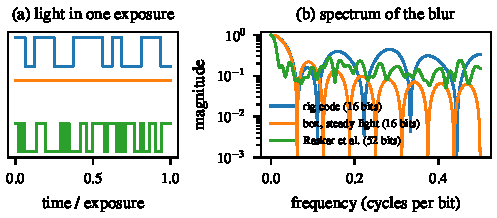
\includegraphics[width=\linewidth]{code_spectrum}
  \caption{(a) The monitor's brightness during one exposure for our rig's code, steady light, and
  the 52-bit code of Raskar et al.~\cite{raskar2006coded}. (b) The magnitude of each blur's spectrum
  (zero-padded DFT, 1 at zero frequency). Steady light has exact zeros, where detail is lost. The
  \rigBits-bit code used for every rig result never falls below \rigMinMTF, and the 52-bit code
  below \raskarMinMTF.}
  \label{fig:code}
\end{figure}

\begin{figure}[t]
  \centering
  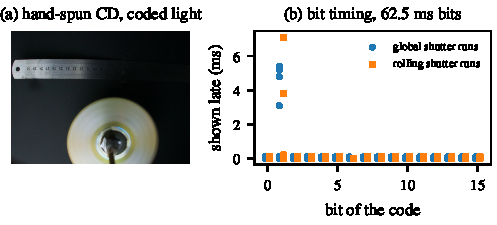
\includegraphics[width=\linewidth]{real_cd}
  \caption{First captures on the rig. (a) A hand-spun CD under coded light (global shutter, processed
  image). The speed varied during the exposure, so these captures cannot be deblurred.
  (b) How late each bit of the code was shown over all \realRuns~coded captures, from the display
  software's log: \realWithinOneMs~of \realBits~bits within \SI{1}{ms}, the worst \realMaxLateMs~ms
  (\realMaxLatePct\% of a bit), always bit \realLateBits.}
  \label{fig:real}
\end{figure}

\Cref{fig:code} compares the codes: steady light has exact spectral zeros, while the 52-bit code
of~\cite{raskar2006coded} keeps every frequency above \raskarMinMTF~of its zero-frequency value and
the \rigBits-bit rig code above \rigMinMTF, so neither loses detail outright. The monitor shows the
code on time: over \realRuns~captures, \realWithinOneMs~of \realBits~bits appeared within \SI{1}{ms}
of schedule (\cref{fig:real}b), the only late one being the first switch to black, at most
\realMaxLateMs~ms (\realMaxLatePct\% of a \realBitMs~ms bit). These times come from the display
software; measured optically (\cref{sec:calibration}), the screen brightens slowly, which the
pipeline models.

\subsection{Simulation: does the pipeline work?}
\label{sec:results-sim}

\begin{figure}[t]
  \centering
  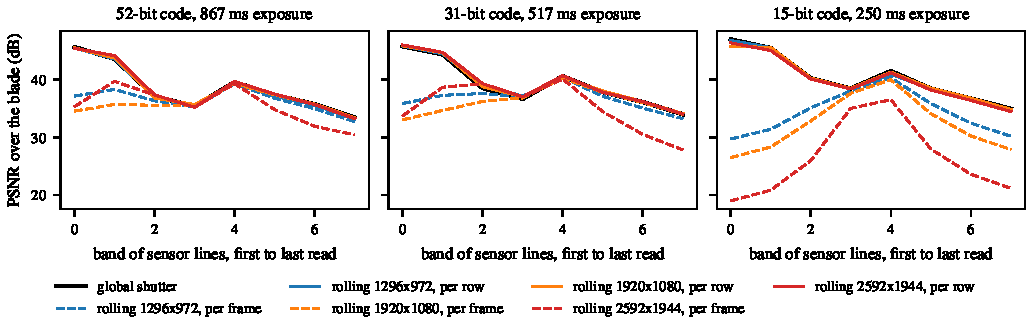
\includegraphics[width=\linewidth]{rows_axis0}
  \caption{Criterion 1 in simulation: image quality by band of sensor lines (first to last read),
  readout down the blade, with the shortest code, where per frame fails most. Black: global shutter;
  solid: per-row rolling shutter for three readout times; dashed: per frame, which falls away from the
  middle band it was timed for (mean \rowsShortFrameMeanA~dB, worst band \rowsShortFrameWorstA~dB,
  against \rowsShortRowMeanA~dB per row at the longest readout). Over all three codes and readouts,
  per row is within \rowsMaxMeanGapA~dB of the global shutter on average and \rowsMaxGapA~dB in its
  worst band. One noise draw per case.}
  \label{fig:rows}
\end{figure}

Simulation showed the pipeline works before any rig data existed. On the harder scene, a photograph
and letters on the blade, DPIR reconstructs the global shutter capture to \psnrGsTex~dB and the per-row
rolling shutter capture to \psnrRsRowTex~dB (\psnrRsFrameTex~dB per frame); steady light gives
\psnrConstTex~dB and a short exposure \psnrShortTex~dB (\cref{tab:solvers}).

\paragraph{Per row against per frame.}
\Cref{fig:rows} tests the first success criterion, per row within \SI{1}{dB} of the global shutter
in every band. Averaged over the frame it is met for every code and readout time; band by band it is
narrowly missed, by up to \rowsMaxGapA~dB in the first bands read, close to the noise of a single
draw. Per frame loses \rowsShortDropA~dB on average against the global shutter with a 15-bit code
and the full sensor readout. With the readout across the blade, per row is within
\rowsMaxMeanGapB~dB on average and \rowsMaxGapB~dB in its worst band.

\paragraph{When does coding pay?}
\Cref{tab:solvers} shows that coding the light pays when the blur is long. At \gainBlurOne~px of blur
steady light deblurs nearly as well (\gainSteadyFullOne~dB against \gainCodedFullOne~dB); at
\gainBlurThree~px coded light gives \gainCodedFullThree~dB against \gainSteadyFullThree~dB. A denoised short
exposure stays below coded light at every blur and light level in the table.

\begin{table}[t]
  \centering\small
  \caption{Simulation, global shutter, PSNR (dB) over the blade. Top: solvers on the two scenes.
  Bottom: coded light against steady light and a denoised short exposure as the blur (at the blade
  tip) grows, DPIR, at full light and at a tenth of the light; a separate noise draw from the top half.}
  \label{tab:solvers}
  % Tikhonov and DPIR: demo.py; the blur rows: coding_gain.py. Both via numbers.tex.
  \setlength{\tabcolsep}{4pt}
  \begin{tabular}{@{}lcc@{}}
    \toprule
    Solver & letters & photograph \\
    \midrule
    Tikhonov, best $\lambda$ & \tikGsLetters & \tikGsTex \\
    DPIR, no tuning & \psnrGsLetters & \psnrGsTex \\
    \midrule
    Blur (coded/steady/short) & full light & a tenth \\
    \midrule
    \gainBlurOne~px & \gainCodedFullOne~/ \gainSteadyFullOne~/ \gainShortFullOne
      & \gainCodedTenthOne~/ \gainSteadyTenthOne~/ \gainShortTenthOne \\
    \gainBlurTwo~px & \gainCodedFullTwo~/ \gainSteadyFullTwo~/ \gainShortFullTwo
      & \gainCodedTenthTwo~/ \gainSteadyTenthTwo~/ \gainShortTenthTwo \\
    \gainBlurThree~px & \gainCodedFullThree~/ \gainSteadyFullThree~/ \gainShortFullThree
      & \gainCodedTenthThree~/ \gainSteadyTenthThree~/ \gainShortTenthThree \\
    \bottomrule
  \end{tabular}
\end{table}

\paragraph{Speed from the photograph.}
The data residual is lowest near the true speed: the estimate is within
\speedErrLetters\% and \speedErrTex\% on the two scenes, against the 5\% target.

\subsection{Rig results}
\label{sec:results-rig}
Every capture was deblurred, none was skipped, and the direction check never flipped a sign.
\Cref{fig:rig-cards} shows the median capture of each set at \SI{\rigCardSpeed}{rpm}. PSNR is
against a still of the stopped fan with the static scene taken out of both (\cref{sec:calibration}),
on the blade picked from the whole capture (margins of at least \rigMarginMin~and \rigRsMarginMin).
With the global shutter camera, coded light deblurs to \rigCodedThree, \rigCodedFive~and
\rigCodedEight~dB at 3, 5 and \SI{8}{rpm}, against \rigSteadyThree, \rigSteadyFive~and
\rigSteadyEight~dB for steady light of the same length deblurred by the same solver: \rigGapMin~to
\rigGapMax~dB better at every speed, by more than the spread between captures
(\cref{fig:rig-psnr}). The rolling shutter camera scores lower, \rigRsCodedThree,
\rigRsCodedFive~and \rigRsCodedEight~dB, but coded light again leads steady light, by \rigRsGapMin~to
\rigRsGapMax~dB. An earlier global shutter session at \SI{3}{rpm} (\rigOctTwentySix~$\pm$ \rigOctTwentySixSd~dB) is
left out: its blades could barely be told apart (margins down to \rigOctTwentySixMarginMin).

\begin{figure}[t]
  \centering
  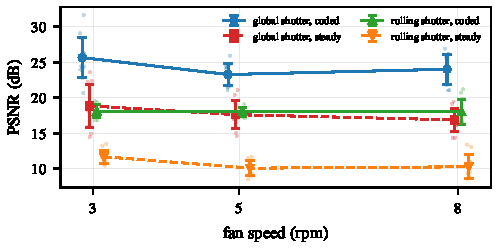
\includegraphics[width=\linewidth]{rig_psnr}
  \caption{The rig: PSNR of the deblurred blades against the stopped fan, coded and steady light of the
  same length, both deblurred with the same solver and monitor model, on both cameras (rolling shutter
  per row). Bars: mean $\pm$ std over 9 to 12 captures; dots: each capture.}
  \label{fig:rig-psnr}
\end{figure}

\paragraph{Criterion 1: per row against the global shutter.} On the rig, per row and per frame gave
identical numbers on all 18 captures run both ways: the padded exposure lets every row see the whole
code (\cref{fig:timing}b), so the per-frame loss of \cref{fig:rows} cannot occur. Band by band the
rolling shutter camera is \rigBandGapMin~to \rigBandGapMax~dB below the global shutter camera
(\rigBandGapMean~dB on average, \cref{fig:rig-rows}), so the \SI{1}{dB} target is missed on the rig.
This compares two cameras, not two corrections: different sensors and lenses, and a blade 1.6 times
larger in the frame, so the same motion smears it over 1.6 times as many pixels.

\begin{figure}[t]
  \centering
  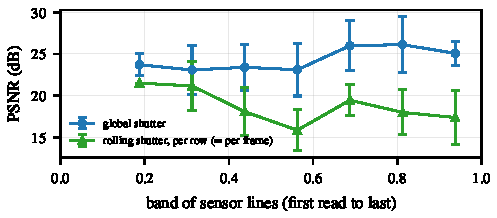
\includegraphics[width=\linewidth]{rig_rows}
  \caption{Criterion 1 on the rig, coded light, every speed: PSNR by band of sensor lines, first read
  to last, mean $\pm$ std over the captures whose blade reached the band. Rolling shutter per row and per
  frame give identical numbers here (padded exposure).}
  \label{fig:rig-rows}
\end{figure}

\paragraph{Criterion 2: letters read.} The still's card read as one of the fan's three letters in
all \rigCardsAll~global and \rigRsCardsAll~rolling shutter captures, and no letter was read from any
capture before deblurring. After deblurring, the global shutter camera read \rigReadCodedThree,
\rigReadCodedFive~and \rigReadCodedEight\% of the letters with coded light at 3, 5 and \SI{8}{rpm},
against \rigReadSteadyThree, \rigReadSteadyFive~and \rigReadSteadyEight\% with steady light
(\cref{fig:rig-criteria}a). The target, at least 90\% with coded light where steady light gives under
50\%, is met at \SI{8}{rpm}; at 3 and \SI{5}{rpm} steady light is still legible. The rolling shutter
camera also reads more with coded light at every speed, but falls short of 90\% at 5 and \SI{8}{rpm}
(\rigReadRsCodedFive~and \rigReadRsCodedEight\%).

\paragraph{Criterion 3: speed from the blur.} With coded light the speed from the blur is within 5\%
of the commanded speed on \rigSpeedWithinCoded~of \rigSpeedAllCoded~global and
\rigSpeedWithinRsCoded~of \rigSpeedAllRsCoded~rolling shutter captures (\cref{fig:rig-criteria}b).
Steady light, whose blur is nearly a plain box, does worse: \rigSpeedWithinSteady~of
\rigSpeedAllSteady~and \rigSpeedWithinRsSteady~of \rigSpeedAllRsSteady~within 5\%.

\begin{figure}[t]
  \centering
  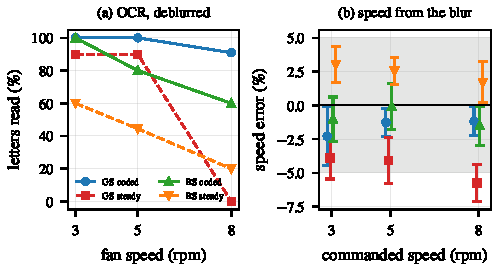
\includegraphics[width=\linewidth]{rig_criteria}
  \caption{The rig, both cameras (GS global, RS rolling shutter). (a) Criterion 2: letters read by OCR
  after deblurring, against the same card on the still. (b) Criterion 3: speed from the blur against the
  commanded speed, mean $\pm$ std; shaded: the $\pm5\%$ target.}
  \label{fig:rig-criteria}
\end{figure}


